\chapter{Introduction}

\section{Big Data: What are they?}

Big Data, as the name suggests, are a collection of huge amount of data, that requires a sophisticated infrastructure to be managed and for its valuable information to be extracted.\newline
It is customary to define Big Data as having three fundamental features known as the 3Vs:

\paragraph{Volume}

The quantity of data generated and stored must be huge, even in the orders of magnitude of the Brontobytes ($10^{27}$ bytes).
Every bit of data might hide some interesting piece of information. The infrastructure must always retrieve as much data as possible and store it for later use.

\paragraph{Velocity}

In the ever changing environment of our digital world, floating in a widespread network linking every device of our life (Internet of Things), data are flowing at an increasing pace. The infrastructure must be able to keep up with this rhythm, as data ages faster each day.

\paragraph{Variety}

With the rapid increase of published information, known as information explosion, data has begun to diversify more and more, and it is now unrealistic to expect just structured textual information such as classical Database tables; the new data flow includes unstructured data such as images, audio, PDFs and raw text files. The infrastructure must be able to extract information from heterogeneous sources.


\section{A Big Data Infrastructure}\label{Chapter2}

As we have established, a Big Data Infrastructure must meet several requirements in order to function properly. 
To manage the complexity needed for this heavy feat, the whole system is organized in several layers; each layer may be implemented with one of several products without changing the rest of the structure.

\begin{figure}
	\centering
	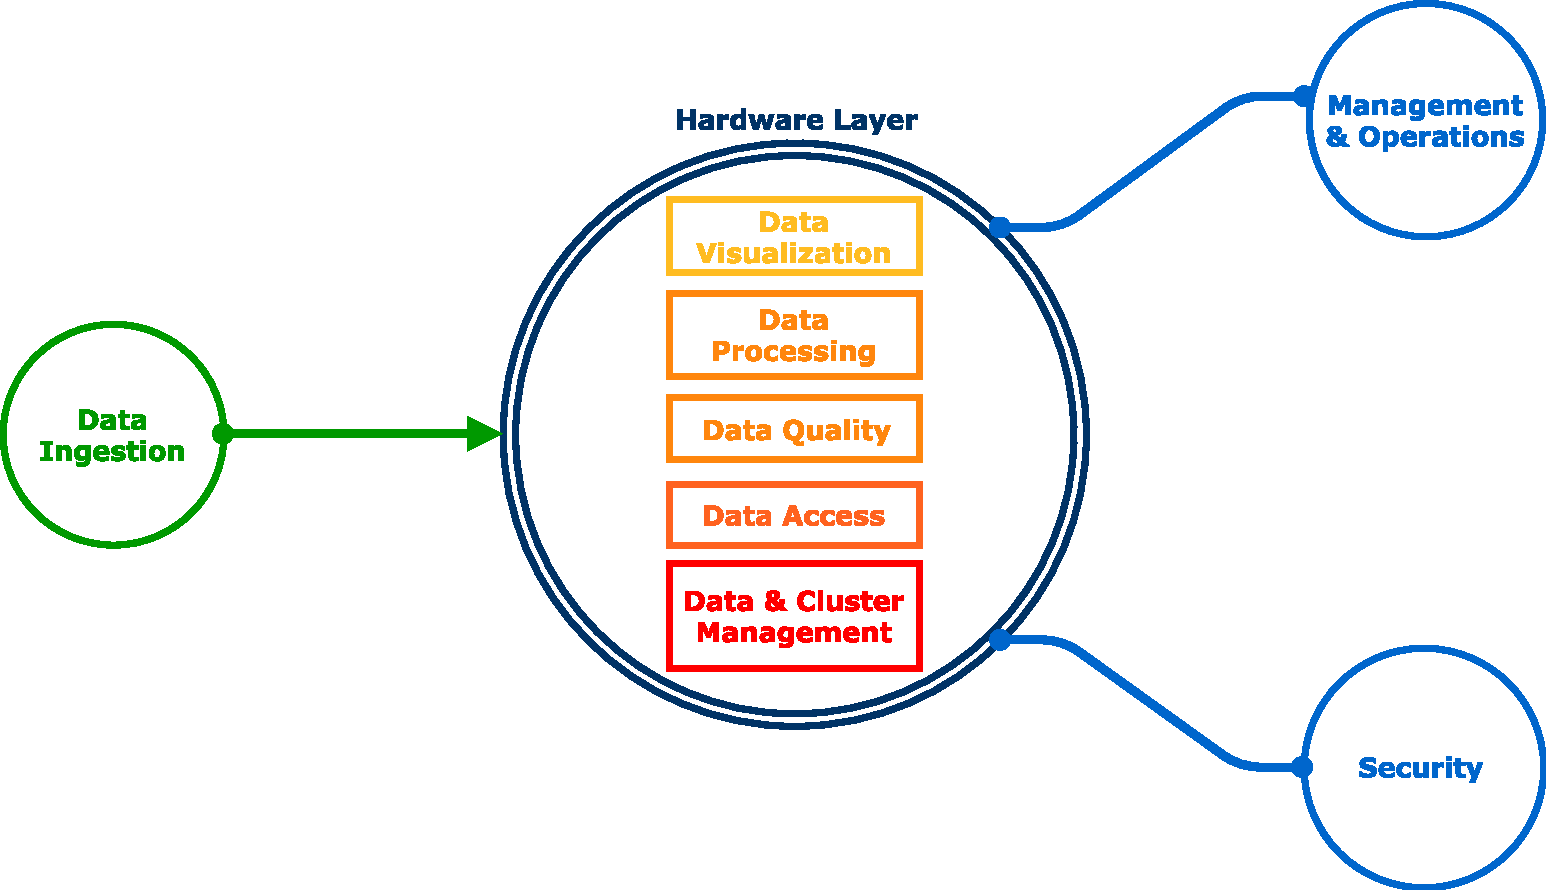
\includegraphics[scale=0.6]{Figures/stack_infrastructure}
	\decoRule
	\caption[Infrastructural Stack]{A model of a Big Data Infrastructure}
	\label{fig:InfrastructuralStack}
\end{figure}

\paragraph{Hardware}

At the foundations of the stack we find the hardware (real or virtualised), which is, in general a group of several machines called a cluster.\newline
The machines are tied together in a single network each to one another, so that communication between them is as easy as possible and the cluster can act like a single machine with high performance and reliability.

\paragraph{Data \& Cluster Management}

Over the first layer of software provided by each machine's Operating System, the cluster needs an interface, so that from an higher point of view, like that of a developer or of an application, the whole system may seem a single entity. \newline
That interface is provided by the Data \& Cluster Management layer, it must offer: 
\begin{itemize}
	\item A distributed File System, able to be accessed like a standard one while providing high fault tolerance thanks to the duplication of data on the different machines of the cluster.
	\item A distributed Operating System, able to manage access to resources on the whole cluster and to schedule application jobs.
\end{itemize}

\paragraph{Data Access}

Having reached a more unified view on the cluster thanks to the previous layer, we can forget about the details of the single machines.\newline
As we would use Databases on a normal computer, so we, on the data access layer, add a distributed Database able to store our data efficiently and for easy access on the distributed File System.
Distributed Databases come in different shapes and styles ranging from the familiar relational ones to non-relational document stores passing through key-value row based stores.

\paragraph{Data Quality}

As mentioned before, our goals are to store as much data as we feasibly can and then process them: the acquisition of big data sets will often lead to a certain amount of dirty data and, what’s more, these huge swaths of data, even cleaned, will be hard to be accessed or made valuable because of their lack of structure.
\newline
Therefore data must go through the Data Quality layer in order to be ready for further processing, this layer must offer applications for:
\begin{itemize}
	\item Data Cleaning, the process of detection, correction and removal of dirty data such as corrupt or wrong records or documents.
	\item Data Wrangling, the process of mapping raw data to a more structured format; wrangling unstructured data also helps their future Cleaning.
\end{itemize}

\paragraph{Data Processing}

Over all the previous strata, we can finally run some applications on the Data Processing layer; those applications, executed in jobs scheduled and managed by the distributed Operating System, process the clean data stored on the distributed Database or on the distributed File System.\newline
This layer provides for distributed processing frameworks where applications can be deployed and run seamlessly on the cluster as a whole, in-memory or on disk, in batches or in real time.\newline
Processed data can then be stored again on the File System or on the Database, formatted or enriched in information for later visualisation or further elaboration.

\paragraph{Data Visualisation}

The topmost layer of the main part of the stack is the Data Visualisation layer which supplies a Visualizing software, whose job is to load data stored on the Database or File System, processed and enriched in the previous layer, and make its information intelligible to humans through the use of images, which can convey several dimensions on a 2D plot thanks to their geometric shape, position and size and their colours.

\paragraph{Data Ingestion}

Orbiting our main stack we find other transversal layers, first among them the Data Ingestion layer.\newline
As described, Big Data infrastructures must be able to handle huge amounts of incoming data at high speed and in real time; this layer provides for applications that can manage incoming real time traffic of data from a source to the cluster, through filtering, mediating and queueing. It might also involve real time cleaning, wrangling and processing applications.

\paragraph{Management \& Operations}

The complexity of the infrastructure with its numerous layers and strong connection between each of them requires an intuitive interface for humans to monitor, manage and maintain the whole infrastructure.\newline
This layer provides a one stop shop for all cluster related operations, showing a dashboard for all the services running on it and supplying an easy way to perform maintenance and updating the system.

\paragraph{Security}

Dulcis in fundo, the valuable information we have extracted thus far, must not be accessible to our competitors or other malicious agents, therefore the cluster must be secured against external attacks.\newline
Also, we need to prevent users from performing operations they are not allowed to perform and to give access to information selectively to each user.
This layer must then provide:
\begin{itemize}
	\item A secure perimeter, so that only authenticated and authorized users might access services on the infrastructure.
	\item Tools for data governance and access control, so that each user is allowed to and only to the data he or she needs.
	\item Tools for auditing so that failed attempts at breaching the perimeter and at performing disallowed operations can be investigated.
\end{itemize}